\chapter{Functional system overview}
based on https://www.inflectra.com/ideas/topic/requirements-definition.aspx

This chapter goes into detail on the functional aspects of the myocardial perfusion phantom.
\section{Drivers}
\label{sec:drivers}
Many factors influence the outcome of \ac{MPI}. Some of these factors are:

\begin{tabular}{llll}
 	\multicolumn{1}{c}{\textbf{Tracer}} & \multicolumn{1}{c}{\textbf{Patient}} & \multicolumn{1}{c}{\textbf{Technology}} & \multicolumn{1}{c}{\textbf{Software}} \\
		- Concentration, & - Breathing artefacts, & - Modality, & - Package, \\
		- Volume, & - Cardiac motion, &  - Spatial resolution, & - Mathematical model, \\
		- Molecule size, & - BMI. & - Temporal resolution. & - Filters,\\
		- Injection speed.  & & & \makecell[l]{- \acs{ROI}.}\\
\end{tabular}

The strength of a phantom is that small modifications, for example, in contrast concentration or volume, or the mathematical model,  can be directly mapped to outcome. It provides insight into dependent and independent factors in perfusion imaging.

Current phantoms either require modifications to software packages or do not model defects in a physiological way. Defects are typically modelled by reducing the flow through the myocardium by reducing the pump rate, effectively ignoring the complex relation between stenotic and non-stenotic arteries. Therefore, a myocardial perfusion phantom is needed that is compatible with clinical software and is able to mimic cardiac defects in a physiological way. This will increase the similarity with patient studies resulting in more reliable validation.

In addition to being a tool for validation of scanners and/or software packages, the phantom can be used for educational and training purposes to demonstrate the impact of hard- and software variables (sampling rate, \acf{ROI}, mathematical model), patient variables (BMI, blood flow and -pressure), tracer variables (concentration, type, injection speed), and many more.

\section{Approach}
The V-Model defines the project's development cycle. 

\subsection{Concept of operations}
\subsection*{Is the D-SPECT's dynamic scanning, in comparison with other modalities (CT, MRI, PET, or SPECT), suitable for quantitative myocardial perfusion imaging?}
Quantitative flow measurements is made possible due to dynamic scanning. Dynamic scanning is not a newly emerged technique, it has been used with \ac{CT} in past research. However, dynamic \ac{SPECT} scanning has recently emerged because of solid-state detectors, i.e. Digirad Cardius, D-SPECT, GE Discovery.

\ac{CT} is a well established modality with the highest spatial resolution. However, its largest drawback is that the radiation dose is directly proportional to the number of images, therefore increasing the likelihood of complication due to radiation exposure. \ac{MRI} does not rely an ionising radiation, but its lower temporal resolution makes it less suitable for dynamic imaging. \ac{SPECT} and \ac{PET} use radioactive tracers to image blood flow, thus exposing the patient to some degree of radiation. However, it is not directly proportional to the amount of images taken and is therefore less dangerous. The new D-SPECT promises significant dose reduction, due to more sensitive solid-state detectors, and better image quality.

In addition, traditional \ac{SPECT} is, on average, 22\% less expensive than the current gold standard, \ac{PET}. D-SPECT is supposed to be less expensive and faster than \ac{SPECT}.

In summary, although dynamic \ac{SPECT} scanning is relatively new, its prospects are promising and potentially suitable for quantitative myocardial perfusion imaging. The D-SPECT has not been properly validated and provides an excellent opportunity to attempt validation of this new modality.

\subsection{What must the myocardial perfusion phantom be able to simulate to validate quantitative MPI?}
At the most basic level, the phantom must be able to create an \ac{AIF}, either via the left ventricle or via an aorta, and simulate the perfusion in the myocardium. Furthermore, the phantom must be able to simulate the complex relation between stenotic and non-stenotic arteries in the myocardium; simply reducing the flow to the entire myocardium is not adequate. It should be possible, in case of simulated stenosis, to visualise the ischaemic tissue along non-ischaemic tissue.

Different kinds of compartment models exist for tracer kinetics. Initially, the phantom should simulate the compartment model consistent with clinical protocol. Additionally, other compartment models should be realisable by, for example, interchanging components.

\section{Business model}
The development of the myocardial perfusion phantom is primarily for the purpose of validating \ac{MPI}. An added benefit is the educational and training purpose. The phantom will distinguish itself from other phantoms due to its more true-to-nature design, ability to physiologically mimic cardiac defects, and the possibility of modelling different compartment models.

The primary focus remains on the current application of \ac{MPI} as performed at the ZGT in Hengelo, Overijssel.

\section{Requirements}
The functional requirements are summarised in table \ref{tab:funcreq}.

\begin{table}
\caption{Functional requirements}
\label{tab:funcreq}
This table summarises the functional requirements for the prototype myocardial perfusion phantom.
\begin{tabular}{l|p{120mm}|}
	\makecell[l]{Requirement \\ number} & \multicolumn{1}{c}{Description}\\
	\hline
	FR01 & The phantom must be able to simulate blood flow, either using water of blood-mimicking fluid, at high flow rates (aortic flow). \\ 
	\rowcolor{Gray}
	FR02 & The phantom must be able to simulate blood flow, either using water or blood-mimicking fluid, at low flow rates (myocardium flow). \\
	FR03 & The high flow should be suitable for an \ac{AIF}, either in a ventricle chamber or an aorta depending on the clinical software. \\
	\rowcolor{Gray}
	FR04 & Cardiac defects should be simulated such that the complex relation between stenotic and non-stenotic arteries is modelled. \\
	FR05 & The phantom must be able to visualise both control and stenotic areas, similar to clinical scans. \\
	\rowcolor{Gray}
	FR06 & The phantom must initially simulate the compartment model typically used in clinical scans, but be flexible enough such that other compartment models are achievable. \\
	FR07 & The contrast agent should be equivalent to that used in clinical scans. \\
	\rowcolor{Gray}
	FR08 & Contrast should be mixed equivalently to contrast mixing in patients. \\
	\cline{2-2}
\end{tabular}
\end{table}

\section{Business and system use cases}	
The myocardial perfusion phantom is primarily used by researchers with varying goals. Primarily, the phantom set-up is a tool to validate perfusion imaging hard- and software and to educate on independent and dependent factors, see section \ref{sec:drivers}. The researcher should be able to adjust the blood flow, both in the myocardium and in the aorta, and be able to set a cardiac defect.

Please note, setting the imaging and contrast parameters are not part of the phantom itself. 
\begin{figure}
	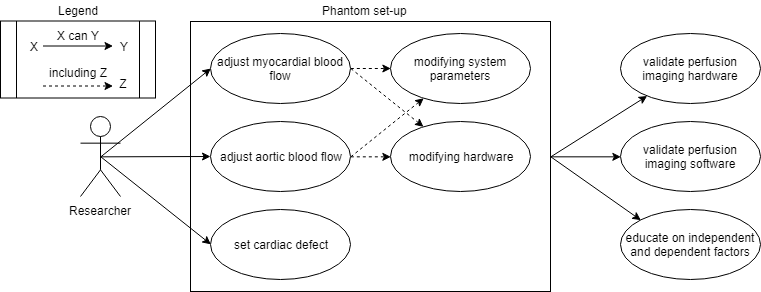
\includegraphics[width=\textwidth]{./images/usecase_diagram.png}
	\caption{Use case diagram for the prototype myocardial perfusion phantom}
	\label{fig:usecase}
\end{figure}

\section{Architectural overview}
A schematic overview of the flow set-up is shown in figure \ref{fig:funcarch}. The set-up consists of a flow generating system, e.g. mechanical pumps or pressure based, to generate the required aortic and myocardial flow, measuring systems, e.g. flow and pressure sensors, and the phantom itself, simulating the heart. The flow is controlled by means of a control system, over which the user has control. The flow parameters, i.e. flow and pressure, are measured by sensors which are monitored by a monitoring system. The monitoring system and control system cooperate such that user parameters are maintained. Figure \ref{fig:funcarch} shows a distinction between high and low flow, which is not a requirement. Low flow can be created by means of pressure difference in high and low flow circuit; increasing pressure in low flow circuit results in less volume passing through.
\begin{figure}
	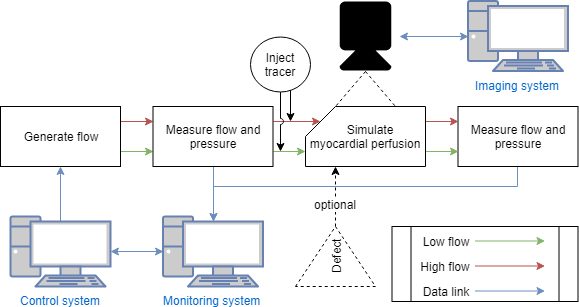
\includegraphics[width=0.75\textwidth]{./images/functional_architecture.png}
	\caption{Functional architecture for the myocardial perfusion set-up}
	\label{fig:funcarch}
\end{figure}
